\documentclass[a4paper,oneside,openany]{tietreport}
\usepackage[T1]{fontenc}
\usepackage{lmodern}
\usepackage{microtype}
\usepackage{float}
\usepackage{array,booktabs,longtable,tabularx}
\usepackage{enumitem}
\usepackage{graphicx}
\graphicspath{{screenshots/}{./}}   % looks in screenshots/ folder, then the main folder
\hypersetup{colorlinks=true,linkcolor=black,citecolor=black,urlcolor=blue}
\setlength{\parindent}{0pt}
\setlength{\parskip}{5pt}
\setlist[itemize]{itemsep=2pt,topsep=3pt}
\setlist[enumerate]{itemsep=2pt,topsep=3pt}
\newcolumntype{Y}{>{\raggedright\arraybackslash}X}
\newcolumntype{L}[1]{>{\raggedright\arraybackslash}p{#1}}
\setlength{\headheight}{14.5pt}
\setlength{\emergencystretch}{2em}
\setlength{\LTpre}{8pt}\setlength{\LTpost}{8pt}
\renewcommand{\arraystretch}{1.15}

%% ---- Title page configuration (tietreport.cls) ----
\TitlePageHeader{%
  UCS 503\\
  Software Engineering Practice Project Report
}

\ProjectTitle{CampusCare}

\ProjectSubTitle{%
  An Integrated Digital Healthcare Platform\\
  for Thapar's Health Center
}

\author{%
  1024030107 & Lavdeep Singh \\
  1024030109 & Harshveer Singh \\
  1024030110 & Damanbir Singh \\
  1024030111 & Kriti%
}

\TitlePageSubText{%
  BE Third Year\\
  Computer Science and Engineering
}

\AdvisorName{Ms. Anushka}

\TitlePageFooterText{%
  \large
  Department of Computer Science and Engineering\\[0.1cm]
  Thapar Institute of Engineering and Technology\\
  Patiala
}
\newcommand{\flowbox}[1]{\fbox{\parbox{.78\linewidth}{\centering\strut #1\strut}}}

% \screenfigure{filename without extension}{caption}
\newcommand{\screenfigure}[2]{%
\begin{figure}[H]\centering
  \IfFileExists{#1.jpg}{%
    \includegraphics[width=\linewidth,height=.36\textheight,keepaspectratio]{#1.jpg}}{%
  \IfFileExists{#1.jpeg}{%
    \includegraphics[width=\linewidth,height=.36\textheight,keepaspectratio]{#1.jpeg}}{%
  \IfFileExists{#1.png}{%
    \includegraphics[width=\linewidth,height=.36\textheight,keepaspectratio]{#1.png}}{%
    \fbox{\parbox[c][15mm][c]{.75\linewidth}{\centering
      Screenshot to be inserted: \texttt{\detokenize{#1}}}}}}}
  \caption{#2}
\end{figure}}

\let\cleardoublepage\clearpage
\begin{document}
\raggedbottom
\maketitle

\tableofcontents
\clearpage

\chapter{Introduction}
\section{Background}
Campus health centres play an important role in providing basic healthcare services to students and staff. On a daily basis, they handle several activities such as student identification, patient registration, queue management, doctor consultations, prescriptions and medicine dispensing. Managing these activities manually can be time-consuming, especially when a large number of students visit the health centre.

Traditional methods, such as paper-based tokens and handwritten prescriptions, can lead to unnecessary waiting, difficulty in tracking queue positions and problems in maintaining previous medical records. Students may not know when their turn will come, while doctors and receptionists may face difficulties in managing patient information efficiently.

To address these problems, CampusCare was developed as an integrated digital healthcare platform specifically designed for Thapar's Health Center. It brings student check-in, doctor-specific queues, medical history, digital prescriptions and medicine dispensing together on a single platform. The system is designed around the existing health centre workflow, which includes two regular doctors, a receptionist responsible for medicine dispensing, an administrator and separate emergency case handling.

By using the existing college ID card for contactless check-in, CampusCare aims to reduce manual work, simplify the consultation process and provide a more organized and convenient healthcare experience for both students and health centre staff.
\section{Problem Statement}

The existing manual system at Thapar's Health Center
presents several challenges for both students and
healthcare staff. The major problems identified are:

\begin{itemize}

    \item \textbf{Lack of Queue Visibility:}
    Students do not have a clear idea of their queue
    position, the number of patients ahead of them
    or when their turn will come.

    \item \textbf{Difficulty in Accessing Medical History:}
    Doctors may face difficulties in retrieving previous
    consultation records and medical information of students.

    \item \textbf{Handwritten Prescriptions:}
    Paper-based prescriptions can be difficult to read,
    easily misplaced and may lead to confusion regarding
    medicine dosage and instructions.

    \item \textbf{Emergency Case Management:}
    Routine consultations and emergency cases require
    different workflows to ensure that urgent cases
    receive appropriate attention.

    \item \textbf{Time-Consuming Registration:}
    Repeated entry of student details and manual token
    management increase the workload of health centre staff.

    \item \textbf{Lack of a Centralized System:}
    Student registration, consultations, prescriptions
    and medicine dispensing are not connected through
    a single digital platform.

\end{itemize}

To overcome these challenges, CampusCare provides an
integrated digital platform that simplifies the entire
process, from student check-in to medicine dispensing.
It uses the existing college ID card for contactless
identification while also providing a manual check-in
option when NFC-based check-in is unavailable.

\section{Motivation}

The main motivation behind CampusCare is to make healthcare
services at Thapar's Health Center more accessible, organized
and convenient for students and staff. Since students already
carry college ID cards with contactless technology, these cards
can be used for quick check-in without the need for additional
cards or paper-based tokens.

Another important motivation is to reduce unnecessary waiting
and manual paperwork. By providing digital queue management,
students can easily check their queue status, while doctors
can access previous medical records and create digital
prescriptions. Receptionists can also manage patient
registration and medicine dispensing more efficiently.

CampusCare aims to bring all these activities together on a
single platform, improving coordination between students,
doctors and health centre staff. The idea is to make better
use of existing technology to solve everyday problems faced
at the campus health centre.
\section{Objectives}
\begin{enumerate}
\item Provide student identification and check-in using the existing college ID card, with a staff-supervised fallback.
\item Maintain independent queues for the two regular doctors.
\item Provide authorized clinicians with relevant student profile and visit history.
\item Record consultations and prescriptions in a structured, retrievable form.
\item Record actual medicine dispensing separately from the prescription.
\item Keep emergency logging outside the routine queue lifecycle.
\item Enforce role-based permissions and maintain an audit trail.
\item Build a maintainable web architecture with a reproducible relational schema.
\end{enumerate}

\section{Scope}
The core scope comprises authentication, student profiles, NFC and manual check-in, doctor availability, doctor-specific queues, no-show handling, redirection, consultation, visit history, Daywise and General prescriptions, dispensing records, emergency logging, administration and audit logging. Medication reminders and anonymized seasonal disease-trend analytics are stretch goals. Inventory management, AI diagnosis, automated triage, payments, insurance, native mobile applications and external hospital/ambulance integration are out of scope.

\section{Existing Workflow and CampusCare Design}
\begin{table}[!htbp]\centering\small
\caption{Comparison of workflows}
\begin{tabularx}{\linewidth}{@{}YYY@{}}\toprule
\textbf{Area} & \textbf{Manual workflow} & \textbf{CampusCare design}\\\midrule
Identification & Manual verification & NFC with manual fallback\\
Queue & Physical tokens & Doctor-specific digital queues\\
Prescription & Handwritten & Structured digital record\\
Dispensing & Manual record & Separate dispensing record\\
History & Fragmented records & Authorized digital retrieval\\
\bottomrule\end{tabularx}\end{table}
\section{Key Innovations}
Reuse of institutional cards, independent doctor queues, preservation of the same encounter during redirection, and separation of prescriptions from dispensing are the central design contributions.

\chapter{Background and Related Concepts}

\section{Contactless Identification}

CampusCare uses the existing college ID card for student
identification and check-in. The card supports ISO/IEC 14443
Type A contactless technology. Using the Web NFC API [1],
a compatible Android device with the Chrome browser reads
the card's unique identifier. The system then matches this
identifier with the registered student in the database.
The card is used only for identification, not for direct
access to medical records.

\section{Web Application Architecture}

CampusCare is developed as a Progressive Web Application
(PWA), allowing users to access it through a browser
without installing a separate mobile application.
React [2] is used to build interactive user interfaces,
Vite supports frontend development, and Tailwind CSS
is used for styling. FastAPI handles backend operations,
while MySQL stores and manages application data.

\section{Authentication and Authorization}

Authentication verifies the identity of a user, while
authorization determines which features the user can access.
Students log in using their institutional Google accounts,
whereas staff members use separately created accounts.
JWT-based authentication and password hashing help protect
staff accounts. Each user can access only the features
and information permitted by their role.

\section{Structured Clinical Information}

CampusCare gives special attention to student health information and patient safety. The system maintains a detailed medical profile for each student, including blood group, emergency contact details, allergies, current medications and existing medical conditions.

Particular importance is given to allergies and ongoing medications, as these can affect the treatment and medicines prescribed by doctors. Doctors can review this information before prescribing medicines, helping them avoid potential allergic reactions and harmful drug interactions. The system also clearly distinguishes between students who have no known allergies and those who have not provided their allergy information.

By keeping important medical information and previous consultation records in one place, CampusCare supports safer and more informed treatment while improving the overall quality of healthcare services.

\section{Technical Foundations}

CampusCare uses a relational database to maintain connections
between students, doctors, visits, prescriptions and
dispensing records. REST APIs enable communication between
the frontend and backend, while JSON Web Tokens (JWT) [3, 4]
help manage authenticated user sessions. FastAPI [5] handles
application requests, and MySQL [6] ensures organized and
consistent data storage.

\section{Related Approaches}

Several existing approaches address individual aspects of
healthcare management. CampusCare aims to bring these
functionalities together on a single platform designed
specifically for a campus health centre.

\begin{table}[htbp]
\centering
\caption{Comparison of Existing Approaches and CampusCare}
\label{tab:related_approaches}
\small
\begin{tabularx}{\textwidth}{XXX}
\toprule
\textbf{Existing Approach} &
\textbf{Limitation} &
\textbf{CampusCare's Solution} \\
\midrule

Paper-based tokens &
Limited queue visibility &
Digital queue tracking \\

Appointment systems &
Limited support for walk-in patients &
Doctor-specific walk-in queues \\

Handwritten prescriptions &
Difficult to read and maintain &
Structured digital prescriptions \\

Contactless identification &
Mainly used for identification &
NFC-based check-in connected to the visit workflow \\

Separate medical records &
Difficulty in accessing previous information &
Centralized student medical history \\

\bottomrule
\end{tabularx}
\end{table}

RFID (Radio Frequency Identification) and NFC (Near Field
Communication) are contactless technologies used for
identification. CampusCare uses NFC to simplify student
check-in while providing a manual alternative for devices
that do not support Web NFC.

\chapter{Requirements Analysis}
\section{Stakeholders and Roles}
\begin{longtable}{@{}L{\dimexpr 0.21805\linewidth-0.87218\tabcolsep\relax}L{\dimexpr 0.45113\linewidth-1.80451\tabcolsep\relax}L{\dimexpr 0.33083\linewidth-1.32331\tabcolsep\relax}@{}}
\caption{CampusCare user roles}\label{tab:roles}\\
\toprule
\textbf{Role}&\textbf{Responsibilities}&\textbf{Restrictions}\\\midrule
\endhead
Student&Authenticate, maintain own profile, check in, select an available doctor, view own queue status, history and prescriptions.&Cannot access another student's records or create prescriptions.\\
Doctor&View own queue, call next student, review relevant history, record consultation, prescribe and redirect a student.&Clinical actions remain server-authorized and attributable.\\
Receptionist&Perform supervised manual check-in, confirm dispensing, record deviations and log standalone emergency cases.&Cannot impersonate the prescriber or overwrite a prescription.\\
Administrator&Manage staff accounts, doctor availability, RFID enrollment/revocation and audit information.&Administrative access does not replace clinical authorship.\\
\bottomrule
\end{longtable}

\section{Functional Requirements}
\begin{longtable}{@{}L{\dimexpr 0.11278\linewidth-0.45113\tabcolsep\relax}L{\dimexpr 0.24060\linewidth-0.96241\tabcolsep\relax}L{\dimexpr 0.64662\linewidth-2.58647\tabcolsep\relax}@{}}
\caption{Functional requirements}\label{tab:fr}\\
\toprule
\textbf{ID}&\textbf{Module}&\textbf{Requirement}\\\midrule
\endhead
FR-01&Student authentication&Authenticate students through the authorized institutional Google identity environment.\\
FR-02&Staff authentication&Authenticate doctor, receptionist and administrator accounts through staff authentication.\\
FR-03&Authorization&Enforce role-specific access in the backend.\\
FR-04&Profile&Allow students to maintain identity, emergency-contact and clinical-safety profile fields.\\
FR-05&NFC check-in&Read an enrolled card on supported Android/Chrome devices and resolve it to a student through CampusCare's credential mapping.\\
FR-06&Manual check-in&Allow an authorized receptionist to identify a student through supervised roll-number lookup.\\
FR-07&Doctor selection&Allow selection of an available doctor.\\
FR-08&Availability&Allow an administrator to mark doctors available or unavailable.\\
FR-09&Queue&Maintain separate queues for each regular doctor and show current student status/position.\\
FR-10&No-show&Mark a missed call as no-show and return the student to the end of the appropriate queue.\\
FR-11&Redirection&Allow a doctor to redirect the same encounter to the other doctor's queue without creating an unrelated duplicate visit.\\
FR-12&Consultation&Allow the doctor to record reason for visit, diagnosis and notes.\\
FR-13&History&Provide authorized access to relevant historical visit and prescription information.\\
FR-14&Prescription&Support structured Daywise medicine entries and General instructions.\\
FR-15&Dispensing&Record actual dispensing separately from the doctor's prescription.\\
FR-16&Emergency&Create emergency records outside the routine queue.\\
FR-17&Administration&Manage staff accounts, availability and RFID enrollment/revocation.\\
FR-18&Audit&Record sensitive actions with actor, action, target and timestamp.\\
\bottomrule
\end{longtable}

\section{Non-Functional Requirements}
\begin{table}[!htbp]\centering\small
\caption{Non-functional acceptance criteria}
\begin{tabularx}{\linewidth}{@{}YYY@{}}\toprule
\textbf{ID} & \textbf{Quality attribute} & \textbf{Acceptance criterion}\\\midrule
NFR-01 & Security & Reject unauthorized record access\\
NFR-02 & Reliability & Prevent duplicate active visits\\
NFR-03 & Usability & Display doctor, position and next action\\
NFR-04 & Maintainability & Use versioned schema migrations\\
NFR-05 & Compatibility & Provide supervised manual fallback\\
NFR-06 & Performance & Measure queue refresh latency under a stated workload\\
\bottomrule\end{tabularx}\end{table}
These criteria define validation targets rather than measured results.

\section{Use Case Diagram}

The use case diagram represents the interaction between
the four main users of CampusCare: Student, Doctor,
Receptionist and Administrator. It shows the different
functionalities available to each user according to
their roles and responsibilities.

\begin{figure}[!htbp]
    \centering
    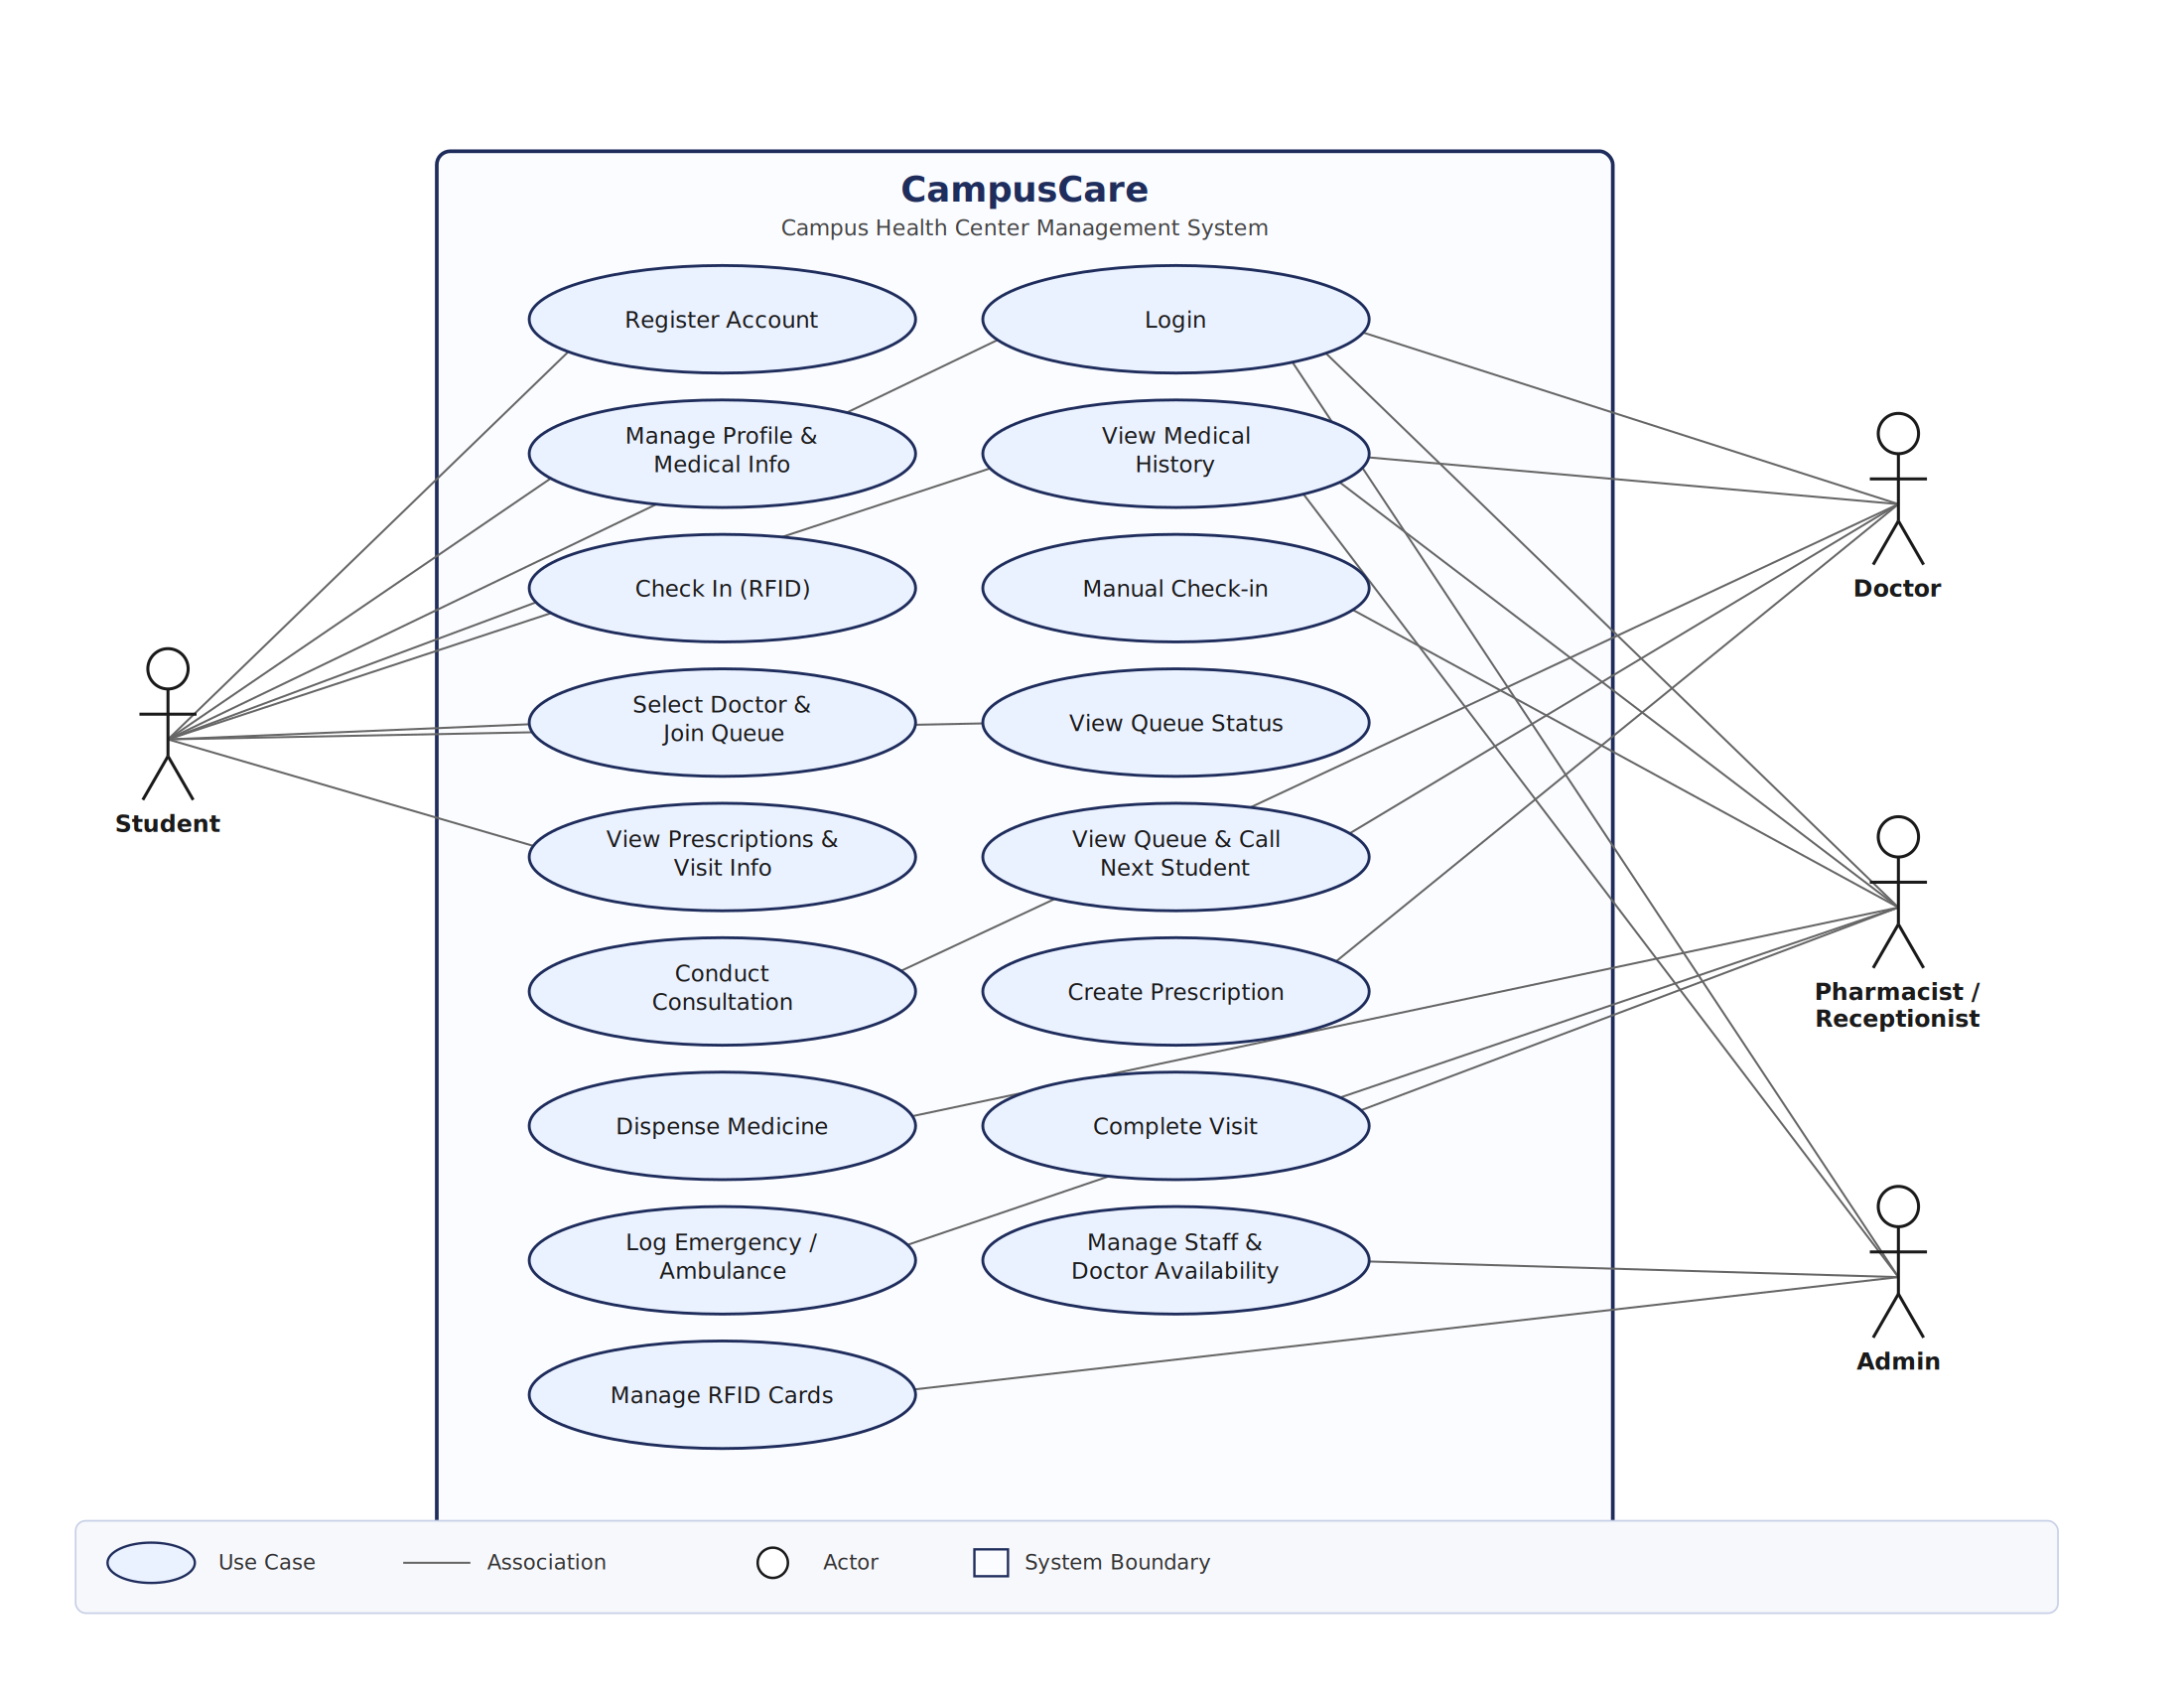
\includegraphics[
        width=0.95\textwidth,
        height=0.65\textheight,
        keepaspectratio
    ]{User_case_dig.png}
    \caption{Use Case Diagram of CampusCare}
    \label{fig:usecase}
\end{figure}
\chapter{System Architecture and Methodology}
\section{Development Methodology}
CampusCare follows a walking-skeleton approach. Development begins with a small end-to-end workflow: manual check-in, one doctor's queue, consultation, prescription and visit completion. The system is then widened to the second queue, redirection, receptionist operations, emergency logging and NFC integration.

\begin{figure}[!htbp]\centering
\resizebox{\linewidth}{!}{\begin{minipage}{\linewidth}\centering\small
\begin{tabular}{c}
\flowbox{0. Design: ERD, state machine, API and wireframes}\\$\downarrow$\\
\flowbox{1. Manual check-in, one queue and consultation}\\$\downarrow$\\
\flowbox{2. Second doctor, dispensing and emergency}\\$\downarrow$\\
\flowbox{3. Polling and concurrency validation}\\$\downarrow$\\
\flowbox{4--5. NFC, administration and audit}\\$\downarrow$\\
\flowbox{6--7. Pilot, hardening and stretch goals}
\end{tabular}
\end{minipage}}
\caption{Walking-skeleton development sequence}\label{fig:method}
\end{figure}

\section{High-Level Architecture}

CampusCare follows a three-tier web architecture consisting
of the frontend, backend and database. Each layer has a
specific responsibility, making the system easier to develop,
test and maintain.

The architecture connects four role-based dashboards with
the FastAPI backend through REST APIs. The backend handles
authentication, request validation and system operations,
while MySQL stores and manages application data. The system
also supports NFC-based identification, institutional Google
login and polling-based queue updates.

Figure~\ref{fig:architecture} illustrates the overall
architecture of CampusCare and the communication between
its different components.

\begin{figure}[H]
    \centering
    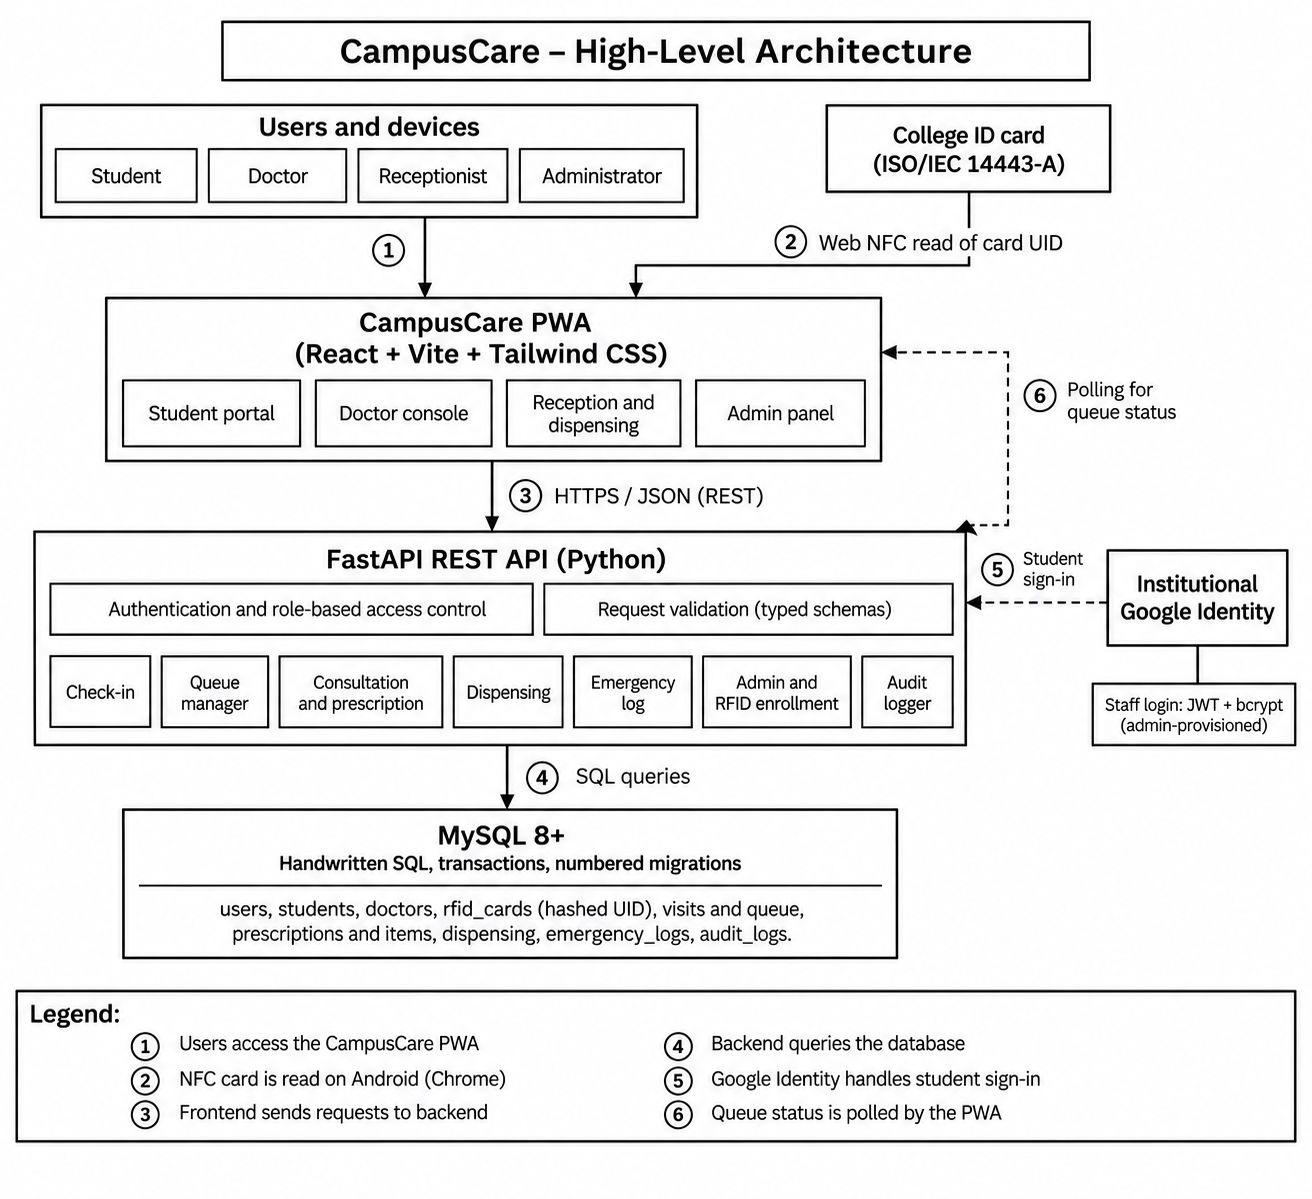
\includegraphics[
        width=\textwidth,
        height=0.70\textheight,
        keepaspectratio
    ]{High_Level_Architecture.jpeg}
    \caption{High-Level Architecture of CampusCare}
    \label{fig:architecture}
\end{figure}

\section{Frontend Layer}
The frontend uses React, Vite, Tailwind CSS and a PWA installation path. Role-specific interfaces support student self-service, doctor queue operations, receptionist dispensing and administration. The design direction is a clinical instrument-panel aesthetic: readable structured data, restrained functional color, flat surfaces and minimal decoration.

\section{Backend Layer}
FastAPI exposes REST endpoints and validates request/response data using typed schemas. Business rules remain on the server. Routes may call database operations directly where appropriate; service abstractions should be introduced when reuse or complexity justifies them.

\section{Database Layer}
MySQL 8+ is the selected database. CampusCare uses handwritten SQL rather than an ORM. Schema evolution is managed through numbered migration files and a migration-tracking table. Applied migrations should not be rewritten casually; subsequent changes should be introduced through new versions.

\section{Authentication}
Students authenticate through the institutional Google identity environment. Staff accounts are administrator-provisioned and use JWT-based authentication with bcrypt password hashing. Authentication and authorization are separate checks.

\chapter{Data Design and Operational Workflows}
\section{Conceptual Data Model}
The principal entities are users, role-specific profiles, RFID credentials, visits, prescriptions, prescription items, dispensing records, emergency logs and audit logs. Supporting normalized structures may represent allergies, chronic conditions, medications, profile history, queue events and visit-state history.

\begin{figure}[!htbp]\centering
\resizebox{\linewidth}{!}{\begin{minipage}{\linewidth}\centering\small
\begin{tabular}{lll}\toprule
\textbf{Parent entity}& &\textbf{Related entity}\\\midrule
USERS & $\longrightarrow$ & AUDIT LOGS\\
USERS & $\longrightarrow$ & STUDENTS, DOCTORS, RECEPTIONISTS\\
STUDENTS & $\longrightarrow$ & RFID CARDS, VISITS\\
DOCTORS & $\longrightarrow$ & VISITS\\
VISITS & $\longrightarrow$ & PRESCRIPTIONS\\
PRESCRIPTIONS & $\longrightarrow$ & PRESCRIPTION ITEMS, DISPENSING\\
RECEPTIONISTS & $\longrightarrow$ & DISPENSING, EMERGENCY LOGS\\\bottomrule
\end{tabular}
\end{minipage}}
\caption{Conceptual entity relationships}\label{fig:erd}
\end{figure}
This figure is conceptual; the exact columns, keys and constraints are defined in the numbered MySQL migration files in the project repository. Emergency logs remain separate from routine visits and queue entries.

\section{Student Medical Profile}
The profile includes full name, roll number, date of birth, sex and contact phone; blood group and emergency contact; structured allergies with reaction and severity; current medications; and selected chronic conditions such as asthma, diabetes, epilepsy/seizure disorder, cardiac condition, thyroid disorder and hypertension. Explicit ``none'' and ``not provided'' states are necessary. Profile changes should preserve historical values rather than silently overwriting previous states.

\section{RFID/NFC Credential Mapping}
The intended flow is: student taps the institutional card; Web NFC reads the card identifier; the client submits it through the protected check-in flow; the backend applies the credential-protection procedure and resolves the credential to a student roll number; the student identity is then associated with the CampusCare account. The credential design requires hashing the UID before storage and avoiding retention of raw card identifiers. The card mapping is maintained within CampusCare and is not an integration with the university's official administrative database. A supervised manual check-in path remains available.

\section{Routine Visit Workflow}
\begin{figure}[!htbp]\centering
\resizebox{\linewidth}{!}{\begin{minipage}{\linewidth}\centering\small
\begin{tabular}{c}
\flowbox{Authentication and card tap / manual verification}\\$\downarrow$\\
\flowbox{Doctor selection and queue entry}\\$\downarrow$\\
\flowbox{Doctor calls student; no-show may rejoin}\\$\downarrow$\\
\flowbox{Consultation and history review}\\$\downarrow$\\
\flowbox{Daywise prescription and General instructions}\\$\downarrow$\\
\flowbox{Dispensing and visit completion}
\end{tabular}
\end{minipage}}
\caption{Routine visit workflow}\label{fig:workflow}
\end{figure}

\section{Doctor-Specific Queues}
Each regular doctor has an independent queue because the doctors are not interchangeable. The student selects an available doctor after identification. The doctor calls the next student from their own queue. If the called student does not appear within a configurable buffer period, the visit is marked no-show and returned to the end of that queue. If the student is in the wrong queue, the doctor can redirect the same encounter to the destination queue's end. Backend transactions must enforce these transitions.
\section{Visit State Machine}

The visit state machine represents the different stages
of a student's visit to the health centre, from initial
check-in to consultation and medicine dispensing.

\begin{figure}[H]
    \centering
    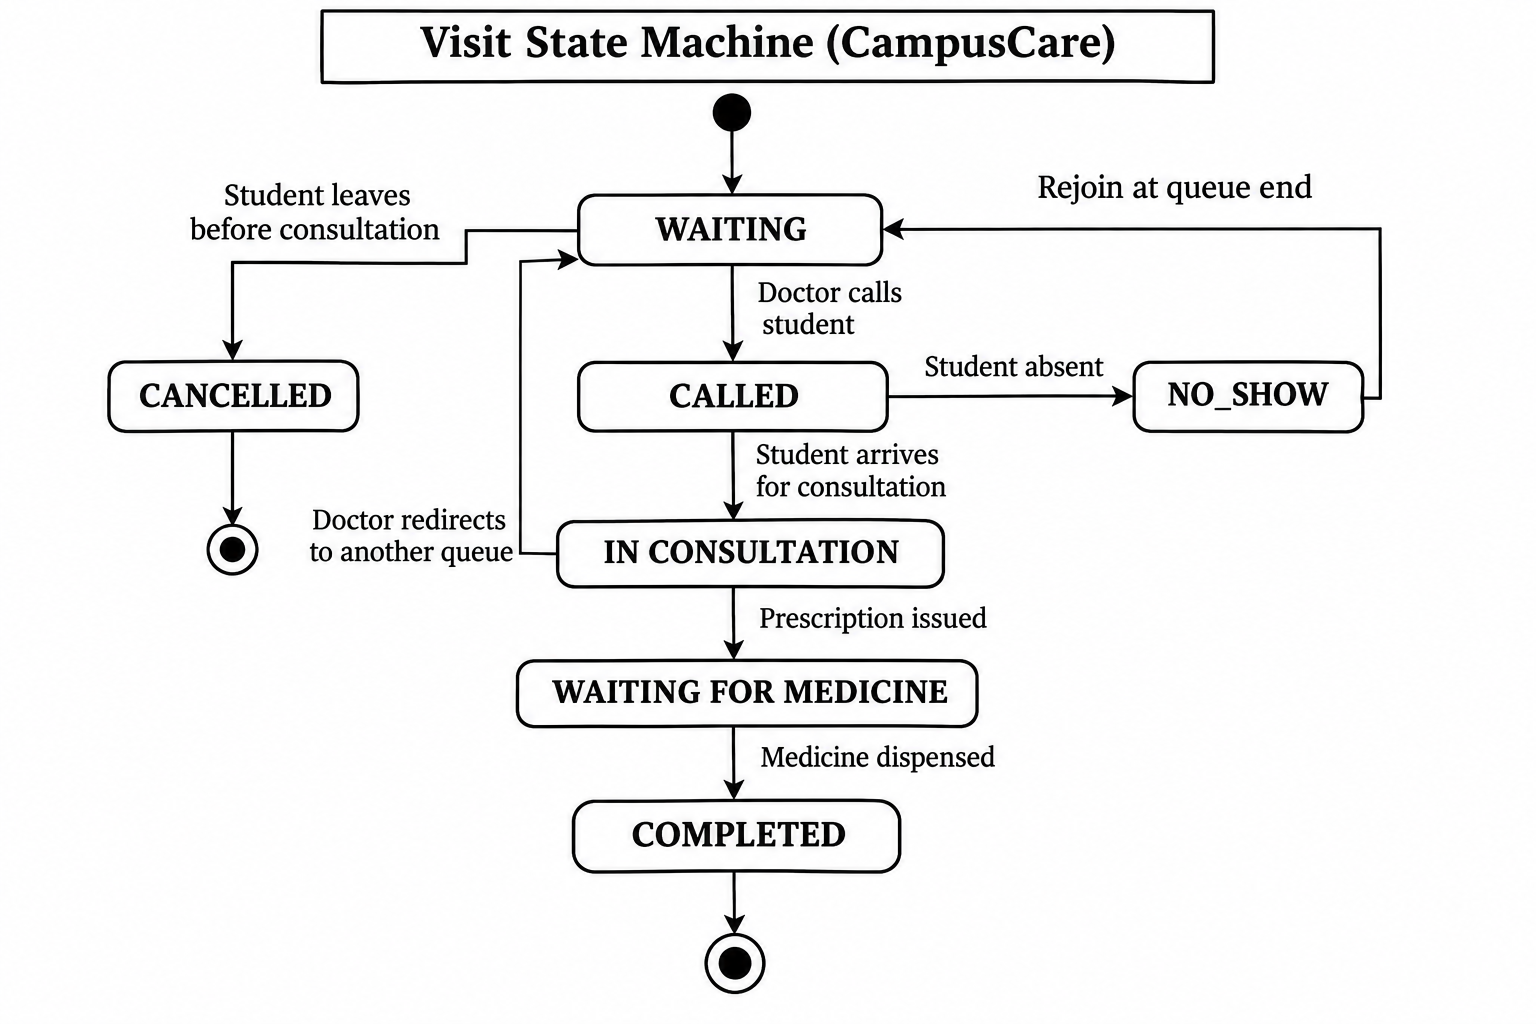
\includegraphics[
        width=\textwidth,
        height=0.65\textheight,
        keepaspectratio
    ]{Visit_State_Machine.png}
    \caption{Visit State Machine of CampusCare}
    \label{fig:state}
\end{figure}

After check-in, the student enters the WAITING state.
When the doctor calls the student, the status changes
to CALLED, followed by IN CONSULTATION once the
consultation begins.

After the prescription is issued, the student moves to
the WAITING FOR MEDICINE state. Once the medicines
are dispensed, the visit is marked as COMPLETED.

If the student is absent when called, the visit is
marked as NO\_SHOW, and the student can rejoin at the
end of the queue. If a student leaves before consultation,
the visit may be marked as CANCELLED.

Doctors can also redirect students to another doctor's
queue without creating a duplicate visit record.
Emergency cases are handled separately from the
routine visit workflow.

\section{Consultation and Prescription}
The doctor records reason for visit, diagnosis and notes, and can review previous visits and relevant medical-profile information. The prescription has two parts: \textbf{Daywise}, structured medicine entries with morning, afternoon and night dosage values, duration and applicable instructions; and \textbf{General}, free-text instructions that do not fit the dose grid.

\section{Prescription and Dispensing Separation}
A prescription is the doctor's clinical instruction. A dispensing record is the receptionist/pharmacist's record of what was actually provided. A substitution or deviation is recorded in dispensing and does not overwrite the original prescription. This preserves clinical authorship and historical traceability.

\section{Standalone Emergency Workflow}
Emergency and trauma cases are logged by the receptionist for the dedicated emergency staff member. They do not require doctor selection, do not enter either regular doctor's queue and do not create a routine queue visit. This separation is structural, not merely a user-interface filter.

\chapter{System Implementation}
\section{Technology Stack}
\begin{longtable}{@{}L{\dimexpr 0.20301\linewidth-0.81203\tabcolsep\relax}L{\dimexpr 0.25564\linewidth-1.02256\tabcolsep\relax}L{\dimexpr 0.54135\linewidth-2.16541\tabcolsep\relax}@{}}
\caption{Selected technology stack}\label{tab:stack}\\
\toprule
\textbf{Layer}&\textbf{Technology}&\textbf{Purpose}\\\midrule
\endhead
Frontend&React, Vite&Component-based browser application and build workflow.\\
Styling&Tailwind CSS&Utility-based interface styling.\\
Application&PWA&Installable web experience; no native app planned.\\
Backend&Python, FastAPI&REST API, validation and application workflows.\\
Database&MySQL 8+&Relational persistence.\\
SQL&Handwritten SQL&Explicit queries and transactions without an ORM.\\
Migrations&Numbered SQL files&Reproducible schema evolution.\\
Student auth&Google identity&Institutional student sign-in.\\
Staff auth&JWT and bcrypt&Staff sessions and password protection.\\
NFC&Web NFC API&Card reading on supported Android/Chrome combinations.\\
Queue refresh&Polling&Initial periodic status refresh.\\
\bottomrule
\end{longtable}

\section{Backend Structure}
The backend is organised as follows:

\begin{center}\begin{minipage}{0.9\linewidth}\small
\begin{verbatim}
backend/
  app/
    main.py
    database.py
    auth.py
    routers/
      checkin.py
      queue.py
      consultation.py
      receptionist.py
      admin.py
  migrations/
    001_init.sql
    002_....sql
  requirements.txt
  .env.example
\end{verbatim}
\end{minipage}\end{center}
The structure can evolve into routes, services and repositories as complexity grows. Business rules affecting identity, queue state, prescriptions or auditability must remain server-side.

\section{Database Design Principles}
A shared users identity table is paired with role-specific profile tables. Exactly one role is assigned to each account. The student's roll number is the institutional identity used by CampusCare. Core entities include users, students, doctors, receptionists, RFID cards, visits, prescriptions, prescription items, dispensing records, emergency logs and audit logs. Supporting tables may hold allergies, conditions, medications, profile history and visit events.

The schema should use primary keys, foreign keys, unique constraints, indexes, non-null constraints and transactions. Medical information should not be stored as comma-separated values when normalized relationships are more appropriate. Migration files are numbered and tracked in a schema-migrations table.

\section{Development Milestones}
The following milestones have been completed:
\begin{itemize}
\item \textbf{NFC proof of concept:} the institutional card identifier was read successfully using an NFC-enabled Android device with Chrome, served over HTTPS from the Vite development server. The card was identified as ISO/IEC 14443-3A (Type A).
\item \textbf{Doctor console:} a React/Tailwind \texttt{DoctorConsole} component covering the doctor queue, patient chart and Daywise prescription grid.
\item \textbf{Landing page:} the CampusCare landing page and sign-in entry point.
\item \textbf{Backend and schema foundation:} the MySQL schema and the FastAPI backend skeleton.
\item \textbf{Role-based interfaces:} the student dashboard, receptionist desk, pharmacy dispensing station, live OPD queue, completed visits view and emergency dispatch interface, shown in Section~\ref{sec:interfaces}.
\end{itemize}
Formal integrated end-to-end testing and production deployment are the remaining steps. The source code is available in the project repository.

\section{Hosting and Development Environment}
Aiven is used as the managed MySQL host during development, Render (or a similar service) is planned for the backend, and Vercel or Netlify for the frontend. DBeaver is used as the database client.

\section{Application Interfaces}\label{sec:interfaces}
The following figures show the CampusCare interfaces, captured using synthetic records.

% Page 1
\screenfigure{Landing_page}{Landing page}
\screenfigure{Login_page}{Authentication and login}

% Page 2
\screenfigure{Student_dashboard}{Student dashboard and queue status}
\screenfigure{NFC}{NFC card identification}

% Page 3
\screenfigure{Doctor_dashboard}{Doctor console}
\screenfigure{E_prescription}{Structured prescription interface}

% Page 4
\screenfigure{Presecption_and_mdeical_history}{Prescription and medical history}
\screenfigure{Reception_dashboard}{Receptionist interface}

% Page 5
\screenfigure{Phramacy_dispensing_station}{Pharmacy dispensing station}
\screenfigure{Emergency_ambulance_dispatch}{Emergency ambulance dispatch interface}

% Page 6
\screenfigure{Live_opd_queue}{Live OPD queue}
\screenfigure{Completed_visits}{Completed visits}

\clearpage

\chapter{System Testing and Results}
\section{Testing Approach}
Testing is organised at unit, integration and end-to-end levels. The objective is to verify identity, visit creation, queue transitions, consultation, prescription and dispensing consistency. Development tests should use synthetic student data. Each case below lists the expected result and the method used to verify it.

\begin{longtable}{@{}L{\dimexpr 0.12403\linewidth-0.74419\tabcolsep\relax}L{\dimexpr 0.22481\linewidth-1.34884\tabcolsep\relax}L{\dimexpr 0.44186\linewidth-2.65116\tabcolsep\relax}L{\dimexpr 0.20930\linewidth-1.25581\tabcolsep\relax}@{}}
\caption{Functional test cases and verification methods}\label{tab:tests}\\
\toprule
\textbf{ID}&\textbf{Area}&\textbf{Expected result}&\textbf{Verification method}\\\midrule
\endhead
TC-01&Student login&Only an authorized institutional identity is accepted.&Manual test in browser\\
TC-02&Staff login&Valid staff credentials establish the correct role; invalid credentials are rejected.&API test (Swagger UI)\\
TC-03&Authorization&Student A cannot retrieve Student B's protected record by changing request parameters.&API test with altered request parameters\\
TC-04&NFC check-in&An enrolled card resolves to the correct student; unknown/revoked cards are rejected.&Web NFC read on Android/Chrome; card-to-student lookup\\
TC-05&Manual check-in&Supervised roll-number verification creates the correct visit.&Manual test as receptionist\\
TC-06&Duplicate visit&A student with an active visit cannot create another active routine visit.&Repeated check-in request\\
TC-07&Availability&An unavailable doctor is not selectable for new routine visits.&Manual test with doctor set unavailable\\
TC-08&Queue ordering&Each doctor has an independent queue and consistent position calculation.&Check-in of multiple students under both doctors\\
TC-09&No-show&A missed call is recorded and the student re-enters at the queue end.&Manual test of call and no-show\\
TC-10&Redirection&Redirecting changes queue assignment without creating a duplicate encounter.&Manual test of redirect\\
TC-11&Consultation&Reason, diagnosis and notes are saved against the correct visit.&Manual test as doctor\\
TC-12&Prescription&Daywise and General information is stored against the consultation.&Manual test; database inspection\\
TC-13&Dispensing&Actual dispensing is recorded separately and does not overwrite prescription.&Manual test as receptionist; database inspection\\
TC-14&Emergency&Emergency logging creates a standalone record without a routine queue entry.&Manual test; database inspection\\
TC-15&Audit&Sensitive changes record actor, action, target and timestamp.&Database inspection of audit table\\
\bottomrule
\end{longtable}

\section{Concurrency and Data Integrity}
Queue operations may be requested simultaneously. The backend must serialize conflicting transitions using database transactions and appropriate row-level locking. Tests should cover simultaneous call-next requests, duplicate check-in attempts, redirect races and concurrent status refreshes. Row-level locking uses MySQL~8 syntax (\texttt{SELECT ... FOR UPDATE}) within transactions.

\section{Security Testing}
Security validation should include expired and invalid tokens, incorrect role access, direct-object-reference attempts, revoked RFID credentials, duplicate active cards, profile-history integrity and audit completeness. The frontend is not a security boundary \cite{owasp}; every protected operation must be checked by the backend.

\section{Evaluation Metrics}

The performance and reliability of CampusCare can be
evaluated using the following criteria:

\begin{itemize}

    \item \textbf{Check-in Time:}
    Time taken to register a student using NFC and
    manual check-in.

    \item \textbf{Queue Accuracy:}
    Correctness of queue positions when multiple
    students check in at the same time.

    \item \textbf{Security:}
    Verification of user login and role-based
    access permissions.

    \item \textbf{Data Consistency:}
    Ensuring that prescription and medicine
    dispensing records match correctly.

    \item \textbf{Response Time:}
    Time taken by the system to process requests
    under different simulated workloads.

    \item \textbf{System Reliability:}
    Ability of the system to recover from interrupted
    requests, network issues or database connection
    failures.

\end{itemize}

These metrics help evaluate the efficiency, accuracy
and reliability of CampusCare. Detailed performance
measurements and large-scale testing can be carried
out in the future.

\chapter{Challenges and Solutions}
\begin{table}[!htbp]\centering\small
\caption{Technical challenges and design responses}
\begin{tabularx}{\linewidth}{@{}YYY@{}}\toprule
\textbf{Challenge} & \textbf{Design response} & \textbf{Verification}\\\midrule
NFC compatibility & Supported Android/Chrome and manual fallback & Card read tested on Android/Chrome\\
Secure context & HTTPS for Web NFC & NFC proof of concept run over HTTPS\\
Duplicate visits & Transactional validation & Test case TC-06\\
Independent queues & Doctor-specific ordering & Test case TC-08\\
Prescription integrity & Separate dispensing record & Test case TC-13\\
Privacy & Role-based access & Test case TC-03\\
\bottomrule\end{tabularx}\end{table}

\chapter{Security, Privacy, Risks and Limitations}
\section{Role-Based Access Control}
CampusCare uses one role per account and enforces permissions in the backend. Students must be restricted to their own records. Staff access should be limited to information necessary for assigned duties and subject to institutional approval and audit controls. The final permission matrix must be verified against actual authorization rules before deployment.

\section{RFID Credential Protection}
The credential protection design requires hashing the card UID before storage and avoiding raw UID persistence. Credential enrollment and revocation are administrative actions and should be audited. A card identifier alone is not sufficient authorization to view health information.

\section{Medical Data Minimization}
The profile collects a limited set of fields relevant to acute care. Sensitive information that is not necessary for the defined workflow is excluded. Development environments should use synthetic records. A real-world pilot involving student health information requires institutional approval, appropriate privacy/security controls and compliance review.

\section{Auditability}
Sensitive actions such as profile updates, RFID enrollment/revocation, doctor-availability changes, consultation amendments and dispensing deviations should create audit records. Audit information should identify actor, action, target record and time, and should not be silently overwritten.

\section{Risks}
\begin{longtable}{@{}L{\dimexpr 0.21805\linewidth-0.87218\tabcolsep\relax}L{\dimexpr 0.36842\linewidth-1.47368\tabcolsep\relax}L{\dimexpr 0.41353\linewidth-1.65414\tabcolsep\relax}@{}}
\caption{Principal risks and mitigations}\label{tab:risks}\\
\toprule
\textbf{Risk}&\textbf{Potential effect}&\textbf{Mitigation}\\\midrule
\endhead
NFC compatibility&Some devices or browsers cannot perform Web NFC reads.&Keep supervised manual check-in and test supported combinations.\\
Network outage&Users may be unable to access queues or records.&Handle errors clearly and maintain operational fallback procedures.\\
Concurrent queue actions&Duplicate calls or inconsistent ordering.&Use server-side state transitions, transactions and database locking.\\
Stale medical profile&Doctor may see outdated allergy or medication information.&Confirm relevant fields during consultation and preserve profile history.\\
Unauthorized access&Exposure of student health information.&Enforce backend authorization, minimize data and audit sensitive access.\\
Incomplete integration&A prototype may be mistaken for a production system.&Report status accurately and complete integration testing before a pilot.\\
\bottomrule
\end{longtable}

\section{Limitations}

Although CampusCare simplifies the daily operations of
the health centre, the system has a few limitations:

\begin{itemize}

    \item \textbf{Device Compatibility:}
    NFC-based check-in works only on supported devices
    and browsers. Students can use manual check-in
    if NFC is unavailable.

    \item \textbf{Queue Management:}
    Some operational rules, such as the waiting time
    before marking a student as absent, still need
    to be finalized.

    \item \textbf{Medical Workflow:}
    Certain details related to doctor specializations
    and prescription fields may require further
    refinement.

    \item \textbf{Queue Updates:}
    The system uses polling to update queue status,
    which may increase the number of requests sent
    to the server.

    \item \textbf{Limited Features:}
    Medicine inventory management, online payments,
    automated diagnosis and automated patient
    prioritization are not included in the current
    system.

    \item \textbf{Mobile Application:}
    CampusCare is a web-based application and does
    not have a separate native mobile application.

    \item \textbf{Performance Testing:}
    Detailed performance testing under real-world
    conditions with a large number of users is yet
    to be conducted.

\end{itemize}

These limitations can be addressed in future versions
to improve the overall performance and functionality
of CampusCare.
\chapter{Conclusion and Future Scope}

\section{Summary of Work}

CampusCare was developed as an integrated digital
healthcare platform for Thapar's Health Centre.
It brings student registration, queue management,
doctor consultation, digital prescriptions and
medicine dispensing together on a single platform.

The main work carried out in this project includes:

\begin{itemize}

    \item \textbf{Role-Based Access:}
    Separate dashboards for students, doctors,
    receptionists and administrators, with secure
    login and access permissions.

    \item \textbf{Contactless Check-in:}
    Student identification using existing college
    ID cards through NFC, along with a manual
    roll-number check-in option.

    \item \textbf{Digital Queue Management:}
    Separate queues for both doctors, including
    no-show handling and student redirection.

    \item \textbf{Student Medical Profile:}
    Access to medical history, allergies, current
    medications and existing health conditions
    during consultations.

    \item \textbf{Digital Prescriptions:}
    Structured prescriptions containing medicine
    dosage, duration and general instructions.

    \item \textbf{Medicine Dispensing:}
    Separate records of medicines prescribed by
    the doctor and medicines actually provided
    to the student.

    \item \textbf{Emergency Management:}
    A separate workflow for emergency cases
    without disturbing the regular consultation
    queue.

    \item \textbf{System Architecture:}
    A three-tier architecture using React, Vite,
    Tailwind CSS, FastAPI and MySQL.

    \item \textbf{System Testing:}
    Preparation of 15 functional test cases to
    evaluate the functionality, security and
    reliability of the system.

\end{itemize}

The project provides a foundation for digitizing
health centre operations. Formal end-to-end testing
and production deployment remain future steps.


\section{Key Findings}

During the design and development of CampusCare,
several important observations were made:

\begin{enumerate}

    \item \textbf{Use of Existing College ID Cards:}
    Existing college ID cards can be used for student
    identification, reducing the need for paper tokens
    or additional cards. However, manual check-in is
    necessary for devices that do not support NFC.

    \item \textbf{Separate Doctor Queues:}
    Maintaining separate queues for each doctor
    helps organize patient visits and allows students
    to be redirected without creating duplicate
    visit records.

    \item \textbf{Separate Prescription and
    Dispensing Records:}
    Maintaining separate records ensures that
    the doctor's original prescription remains
    unchanged, even if there are changes during
    medicine dispensing.

    \item \textbf{Importance of Medical Information:}
    Providing doctors with information about allergies,
    current medications and medical history supports
    safer and better-informed treatment decisions.

    \item \textbf{Backend Security and Validation:}
    Important operations must be controlled by the
    backend to prevent unauthorized access, duplicate
    visits and incorrect queue updates.

    \item \textbf{Separate Emergency Workflow:}
    Managing emergency cases separately helps prevent
    interference with routine consultations and
    supports appropriate handling of urgent cases.

\end{enumerate}

These findings highlight the importance of designing
a healthcare system around the actual requirements
of its users.


\section{Future Work and Recommendations}

CampusCare can be further improved by introducing
the following features and enhancements:

\begin{enumerate}

    \item \textbf{System Testing and Performance
    Evaluation:}
    Conduct detailed end-to-end testing and measure
    system performance when multiple users access
    the platform simultaneously.

    \item \textbf{Health Centre Integration:}
    Introduce CampusCare at Thapar's Health Centre
    on a trial basis after obtaining institutional
    approval and completing the required security
    and privacy checks.

    \item \textbf{Real-Time Queue Updates:}
    Replace polling with WebSockets to provide
    faster queue updates and reduce unnecessary
    server requests.

    \item \textbf{Workflow Improvements:}
    Finalize any remaining rules related to no-show
    handling, doctor specializations, prescription
    fields and user permissions.

    \item \textbf{Production Deployment:}
    Deploy the system on a reliable hosting platform
    and improve its ability to handle network and
    database failures.

    \item \textbf{Medication Reminders:}
    Provide reminders to students to help them
    take prescribed medicines on time.

    \item \textbf{Health Analytics:}
    Use anonymized medical records to identify
    common illnesses and seasonal health trends
    within the campus.

    \item \textbf{Medicine Inventory Management:}
    Maintain medicine stock records and notify staff
    when medicines are running low.

\end{enumerate}


\section{Final Remarks}

CampusCare aims to make healthcare services at
Thapar's Health Centre more organized, accessible
and efficient. By connecting student identification,
queue management, consultations, prescriptions and
medicine dispensing, the system addresses several
difficulties associated with manual healthcare
operations.

The project also gives importance to patient safety,
data privacy and secure access to medical information.
With further testing, improvements and institutional
integration, CampusCare has the potential to provide
a better healthcare experience for both students
and health centre staff.
\renewcommand{\bibname}{References}
\phantomsection
\addcontentsline{toc}{chapter}{References}

\begin{thebibliography}{99}

\bibitem{nfc_docs}
Mozilla, ``Web NFC API,''
\textit{MDN Web Docs}.
[Online]. Available:
\url{https://developer.mozilla.org/en-US/docs/Web/API/Web_NFC_API}.

\bibitem{react_docs}
React, ``React Documentation.''
[Online]. Available:
\url{https://react.dev/}.

\bibitem{fielding2000}
R. T. Fielding,
\textit{Architectural Styles and the Design of
Network-based Software Architectures},
Ph.D. dissertation, University of California,
Irvine, 2000.
[Online]. Available:
\url{https://ics.uci.edu/~fielding/pubs/dissertation/top.htm}.

\bibitem{rfc7519}
M. Jones, J. Bradley, and N. Sakimura,
``JSON Web Token (JWT),''
RFC 7519, May 2015.
[Online]. Available:
\url{https://www.rfc-editor.org/rfc/rfc7519}.

\bibitem{fastapi_docs}
S. Ramirez, ``FastAPI Documentation.''
[Online]. Available:
\url{https://fastapi.tiangolo.com/}.

\bibitem{mysql_docs}
Oracle Corporation, ``MySQL 8.0 Reference Manual.''
[Online]. Available:
\url{https://dev.mysql.com/doc/refman/8.0/en/}.

\bibitem{owasp}
OWASP Foundation,
``OWASP Top 10: Web Application Security Risks.''
[Online]. Available:
\url{https://owasp.org/www-project-top-ten/}.

\bibitem{vite_docs}
Vite, ``Vite Documentation.''
[Online]. Available:
\url{https://vite.dev/guide/}.

\bibitem{tailwind_docs}
Tailwind Labs, ``Tailwind CSS Documentation.''
[Online]. Available:
\url{https://tailwindcss.com/docs}.

\bibitem{google_identity}
Google, ``Google Identity Services.''
[Online]. Available:
\url{https://developers.google.com/identity}.

\bibitem{pwa_docs}
Mozilla, ``Progressive Web Apps (PWAs),''
\textit{MDN Web Docs}.
[Online]. Available:
\url{https://developer.mozilla.org/en-US/docs/Web/Progressive_web_apps}.

\bibitem{iso14443}
International Organization for Standardization,
\textit{Cards and Security Devices for Personal
Identification -- Contactless Proximity Objects --
Part 3: Initialization and Anticollision},
ISO/IEC 14443-3:2018, 2018.

\bibitem{password_security}
OWASP Foundation,
``Password Storage Cheat Sheet.''
[Online]. Available:
\url{https://cheatsheetseries.owasp.org/cheatsheets/Password_Storage_Cheat_Sheet.html}.

\end{thebibliography}

\end{document}